\section{Funcionamento do Oculus Rift}
Colocar aqui como o Oculus Rift define os valores gerados, como eh feita a distorcao, como eh feito o calculo de customizacao para pessoas com diferentes distancia entre os olhos e talz

\subsection{Esquema de coordenadas}
Falar do esquema de coordenadas do Oculus rift. Traduzir:
As seen from the diagram, the coordinate system uses the follow-
ing axis definitions:
\begin{itemize}
	\item Y eh positivo para cima
	\item X eh positivo para direita
	\item Z eh positivo para tras
\end{itemize}
Rotation is maintained as a unit quaternion, but can also be
reported in yaw-pitch-roll form. Positive rotation is counter-
clockwise (CCW, direction of the rotation arrows in the diagram)
when looking in the negative direction of each axis, and the com-
ponent rotations are:
\begin{itemize}
	\item Pitch is rotation around X, positive when pitching up.
	\item Yaw is rotation around Y , positive when turning left.
	\item Roll is rotation around Z, positive when tilting to the left in the XY plane.
\end{itemize}

\begin{figure}[h]
  \centering
  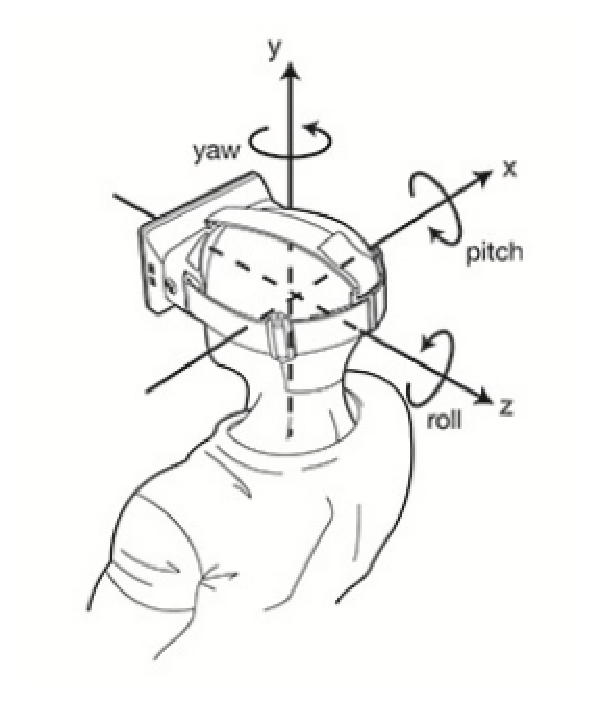
\includegraphics[width=0.5\textwidth]
      {figuras/esquema_coordenadas_rift.eps}
  \caption{Esquema de coordenadas do Oculus Rift}
  \label{coordenadas-rift}
\end{figure}

\subsection{Distorcao}
Falar aqui um pouco sobre as distorcoes da lente e das imagens. Traduzir:
The Oculus Rift requires the scene to be rendered in split-screen stereo with half the screen used for each
eye. When using the Rift, the left eye sees the left half of the screen, and the right eye sees the right half.
Although varying from person-to-person, human eye pupils are approximately 65 mm apart. This is known
as interpupillary distance (IPD). The in-application cameras should be configured with the same separation.
Note that this is a translation of the camera, not a rotation, and it is this translation (and the parallax effect
that goes with it) that causes the stereoscopic effect. This means that your application will need to render the
entire scene twice, once with the left virtual camera, and once with the right.
Note that the reprojection stereo rendering technique, which relies on left and right views being generated
from a single fully rendered view, is usually not viable with an HMD because of significant artifacts at object
edges.
The lenses in the Rift magnify the image to provide a very wide field of view (FOV) that enhances immersion.
However, this process distorts the image significantly. If the engine were to display the original images on the
Rift, then the user would observe them with pincushion distortion.
To counteract this distortion, the software must apply post-processing to the rendered views with an equal
and opposite barrel distortion so that the two cancel each other out, resulting in an undistorted view for each
eye. Furthermore, the software must also correct chromatic aberration, which is a rainbow effect at the edges
caused by the lens. Although the exact distortion parameters depend on the lens characteristics and eye
position relative to the lens, the Oculus SDK takes care of all necessary calculations when generating the
distortion mesh.
When rendering inside the Rift, projection axes should be parallel
to each other as illustrated in Figure 5, and the left and right views
are completely independent of one another. This means that
camera setup is very similar to that used for normal non-stereo
rendering, except that the cameras are shifted sideways to adjust
for each eye location.
In practice, the projections in the Rift are often slightly off-center
because our noses get in the way! But the point remains, the left
and right eye views in the Rift are entirely separate from each
other, unlike stereo views generated by a television or a cinema
screen. This means you should be very careful if trying to use
methods developed for those media because they do not usually
apply to the Rift.
Figure 5: HMD eye view cones.
The two virtual cameras in the scene should be positioned so that they are pointing in the same direction
(determined by the orientation of the HMD in the real world), and such that the distance between them is the
same as the distance between their eyes, or interpupillary distance (IPD). This is typically done by adding the
ovrEyeRenderDesc::ViewAdjust translation vector to the translation component of the view matrix.
Although the Rift’s lenses are approximately the right distance apart for most users, they may not exactly
match the user’s IPD. However, because of the way the optics are designed, each eye will still see the correct
view. It is important that the software makes the distance between the virtual cameras match the user’s IPD
as found in their profile (set in the configuration utility), and not the distance between the Rift’s lenses.

\begin{figure}[h]
  \centering
  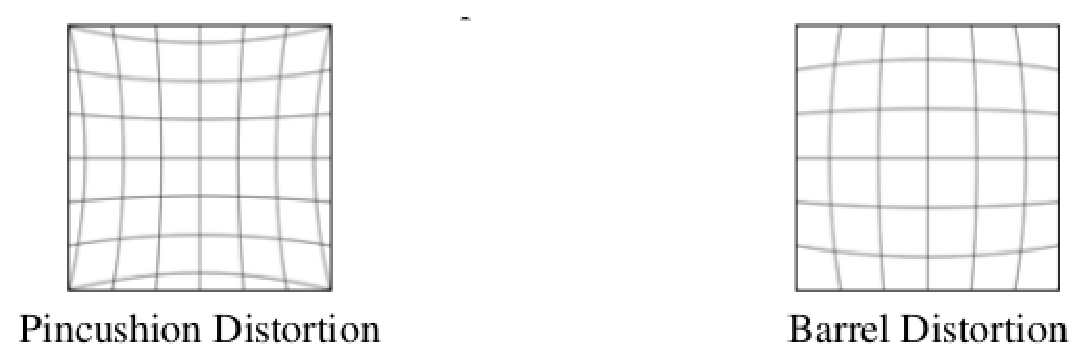
\includegraphics[width=0.7\textwidth]
      {figuras/distorcao_rift.eps}
  \caption{Distorcao de lentes e imagens do Rift}
  \label{coordenadas-rift}
\end{figure}

